\documentclass[11pt]{article}

\usepackage[margin=1in]{geometry}
\usepackage{amsmath}
\usepackage{booktabs}
\usepackage{float}
\usepackage{graphicx}
\usepackage{hyperref}
\usepackage[numbers]{natbib}

\title{Modeling the First COVID-19 Wave in Hubei with a Simple SIR Model}
\author{Bohan Yin}
\date{May 2026}

\begin{document}
\maketitle

\begin{abstract}
This project uses susceptible-infected-removed (SIR) models to study the first reported COVID-19 wave in Hubei, China. Using Johns Hopkins CSSE cumulative confirmed case data from January 22, 2020 to April 30, 2020, I first fit a constant-transmission SIR model and then extend it to allow the transmission rate $\beta(t)$ to decline over time. The constant-$\beta$ model gives $\beta \approx 0.329$, $\gamma \approx 0.065$, and effective population size $N_{\mathrm{eff}} \approx 68{,}809$. The time-varying model improves the fit and estimates a decline in transmission around February 15, 2020. I also use the fitted constant-$\beta$ model to test hypothetical reductions in transmission. These results support the general ``flattening the curve'' idea, while also showing the limitations of applying simple SIR models to reported COVID-19 case data.
\end{abstract}

\section{Introduction}

Compartment models are a common way to study infectious disease dynamics. In an SIR model, the population is divided into susceptible, infected, and removed individuals, and the flow between these groups is described by differential equations. Cooper, Mondal, and Antonopoulos used an SIR-type model to study COVID-19 spread in different communities, showing how a relatively simple model can still give insight into epidemic growth and control \cite{cooper2020sir}.

The scientific question in this project is:

\begin{quote}
Can a simple SIR model approximate the first COVID-19 wave in Hubei, and how does allowing the transmission rate to change over time affect the model's interpretation?
\end{quote}

I focus on Hubei because it was the center of the earliest large COVID-19 outbreak in China and because province-level time series data are available in a clean form. The goal is not to build a complete COVID-19 forecasting model. Instead, the goal is to test how much can be learned from a basic SIR model, then ask whether a more realistic time-varying transmission rate improves the explanation.

\section{Data}

The data come from the Johns Hopkins CSSE COVID-19 time series repository \cite{jhu2020data}. I use the global confirmed cases file and select the row with province/state equal to Hubei and country/region equal to China. The time period is January 22, 2020 through April 30, 2020, which captures the first reported wave in Hubei.

The original dataset reports cumulative confirmed cases by date. I also compute daily new cases by differencing the cumulative counts. Figure \ref{fig:daily} shows the reported daily new cases. One noticeable feature is the large reporting jump in mid-February 2020. This is important because the model is smooth, but reported data can change suddenly due to testing capacity or case definition changes.

\begin{figure}[H]
    \centering
    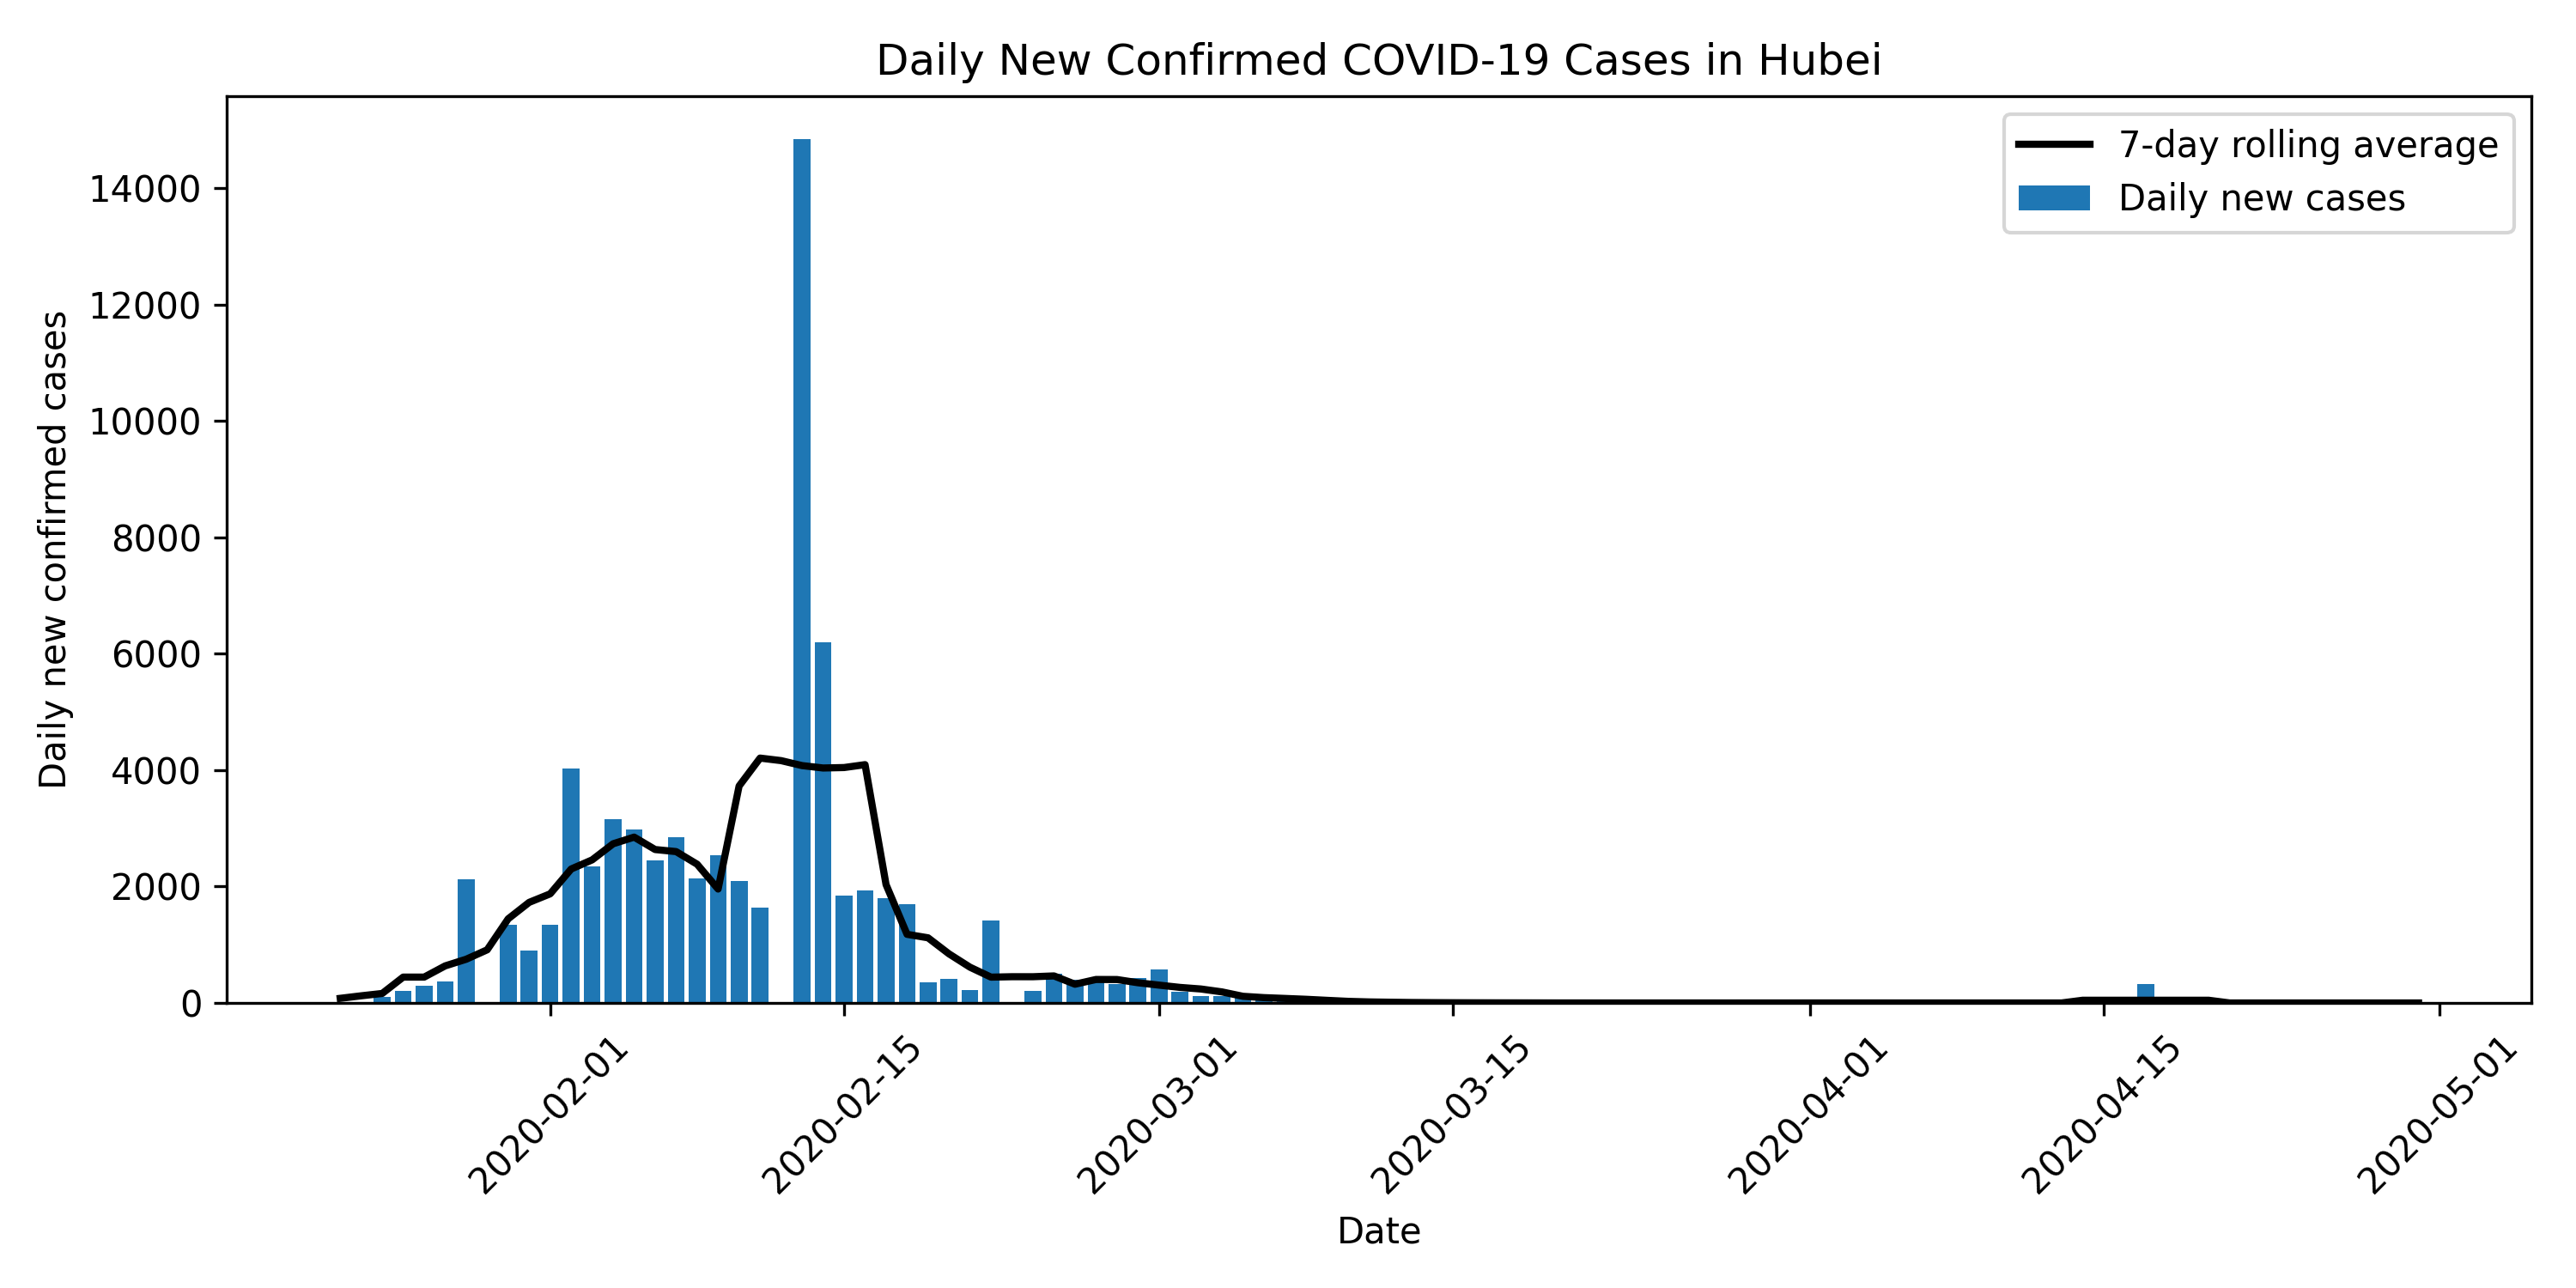
\includegraphics[width=0.9\textwidth]{figures/hubei_daily_cases.png}
    \caption{Daily new confirmed COVID-19 cases in Hubei from January 22, 2020 to April 30, 2020. The black curve shows a 7-day rolling average.}
    \label{fig:daily}
\end{figure}

\section{Model}

The baseline model is the standard SIR system
\begin{align}
    \frac{dS}{dt} &= -\beta \frac{SI}{N}, \\
    \frac{dI}{dt} &= \beta \frac{SI}{N} - \gamma I, \\
    \frac{dR}{dt} &= \gamma I.
\end{align}

Here $S(t)$ is the susceptible population, $I(t)$ is the infected population, $R(t)$ is the removed or recovered population, and $N$ is the effective population size used in the model. The parameter $\beta$ is the transmission rate, and $\gamma$ is the removal rate. The basic reproduction number in this simple model is
\begin{equation}
    R_0 = \frac{\beta}{\gamma}.
\end{equation}

The cumulative number of infections generated by the model is
\begin{equation}
    C(t) = N - S(t).
\end{equation}
I fit this model-generated cumulative case count to the reported cumulative confirmed cases.

The main extension replaces the constant transmission rate with a time-varying transmission rate:
\begin{equation}
    \beta(t) = \beta_{\mathrm{low}} + \frac{\beta_0 - \beta_{\mathrm{low}}}{1 + e^{(t-t_c)/w}},
\end{equation}
where
\begin{equation}
    \beta_{\mathrm{low}} = m\beta_0.
\end{equation}
Here $\beta_0$ is the early transmission rate, $m$ is the fraction of the early transmission rate that remains after the decline, $t_c$ is the midpoint of the transition, and $w$ controls how quickly the transition occurs. This form keeps $\beta(t)$ positive and allows the model to represent a smooth decrease in effective transmission over time.

\section{Methods}

I solved the SIR differential equations numerically using Python's \texttt{solve\_ivp}. For the constant-$\beta$ model, the fitted parameters were $\beta$, $\gamma$, and an effective population size $N_{\mathrm{eff}}$. For the time-varying model, the fitted parameters were $\beta_0$, $m$, $t_c$, $w$, $\gamma$, and $N_{\mathrm{eff}}$. I used least squares optimization to minimize the scaled difference between the model cumulative cases and the reported cumulative confirmed cases.

After fitting the baseline model, I also ran four transmission scenarios:
\[
    \beta,\quad 0.9\beta,\quad 0.8\beta,\quad 0.7\beta.
\]
These represent the fitted transmission rate and hypothetical 10\%, 20\%, and 30\% reductions in transmission. For each scenario, I recorded the peak model daily cases, the date of the peak, and the final cumulative cases over the study period.

\section{Results}

The constant-$\beta$ fitted parameter values were
\[
    \beta = 0.32884,\qquad
    \gamma = 0.06530,\qquad
    R_0 = 5.04,\qquad
    N_{\mathrm{eff}} = 68{,}809.
\]
The value of $N_{\mathrm{eff}}$ should not be interpreted as the full population of Hubei. It is an effective population size for the reported first-wave outbreak under this simplified model.

Figure \ref{fig:fit} compares the fitted SIR cumulative case curve with the reported cumulative confirmed cases. The model captures the broad S-shaped pattern of the first wave, but it does not capture abrupt reporting changes exactly.

\begin{figure}[H]
    \centering
    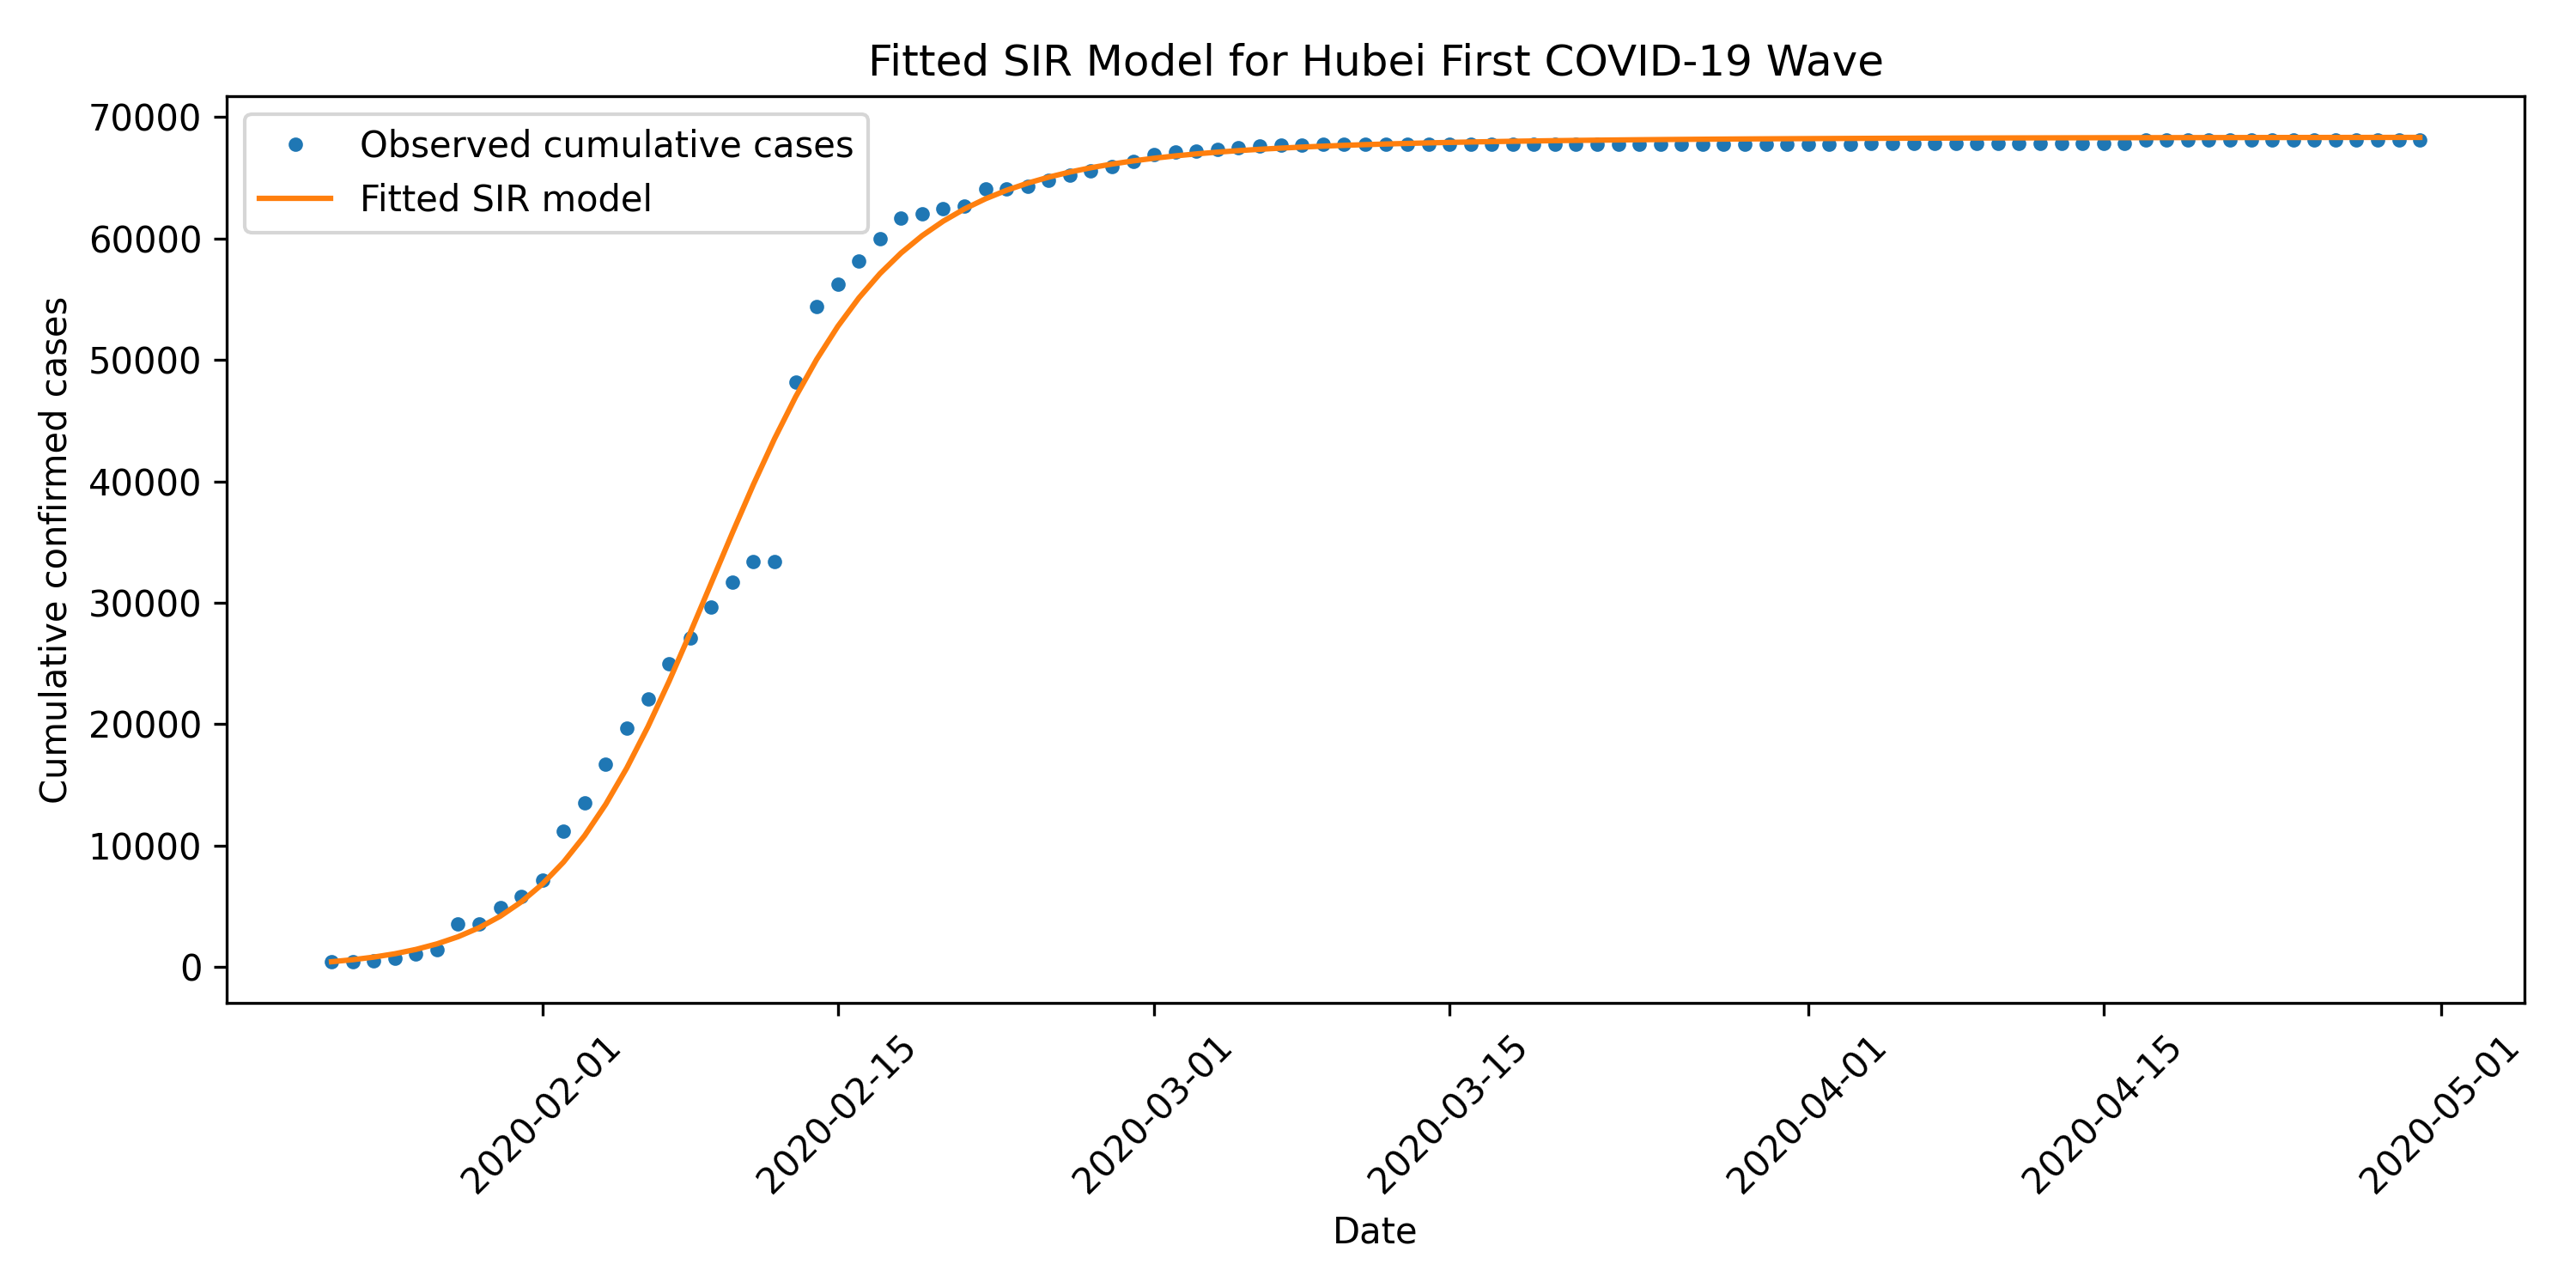
\includegraphics[width=0.9\textwidth]{figures/hubei_sir_fit.png}
    \caption{Fitted SIR model compared with observed cumulative confirmed cases in Hubei.}
    \label{fig:fit}
\end{figure}

The time-varying transmission model improved the scaled least squares fit cost from $0.0301$ to $0.0197$. The fitted parameters were
\[
    \beta_0 = 0.810,\qquad
    m = 0.657,\qquad
    t_c = 23.7,\qquad
    w = 1.0,\qquad
    \gamma = 0.652.
\]
Since day 0 is January 22, 2020, the fitted transition midpoint corresponds to about February 15, 2020. Under this model, $\beta(t)$ decreases from about $0.810$ early in the outbreak to about $0.532$ by the end of the study period. The corresponding ratio $\beta(t)/\gamma$ decreases from about $1.24$ to about $0.82$.

\begin{figure}[H]
    \centering
    
\includegraphics[width=0.9\textwidth]{figures/hubei_constant_vs_time_varying_sir_fit.png}
    \caption{Comparison of the constant-$\beta$ SIR fit and the time-varying $\beta(t)$ SIR fit.}
    \label{fig:timevaryingfit}
\end{figure}

\begin{figure}[H]
    \centering
    
\includegraphics[width=0.9\textwidth]{figures/hubei_time_varying_beta.png}
    \caption{Estimated time-varying transmission rate $\beta(t)$ from the logistic-decline SIR model.}
    \label{fig:betat}
\end{figure}

The counterfactual simulations show that lowering the transmission rate reduces the peak number of model daily cases and delays the peak. Figure \ref{fig:counterfactual} shows the daily case curves under each transmission scenario.

\begin{figure}[H]
    \centering
    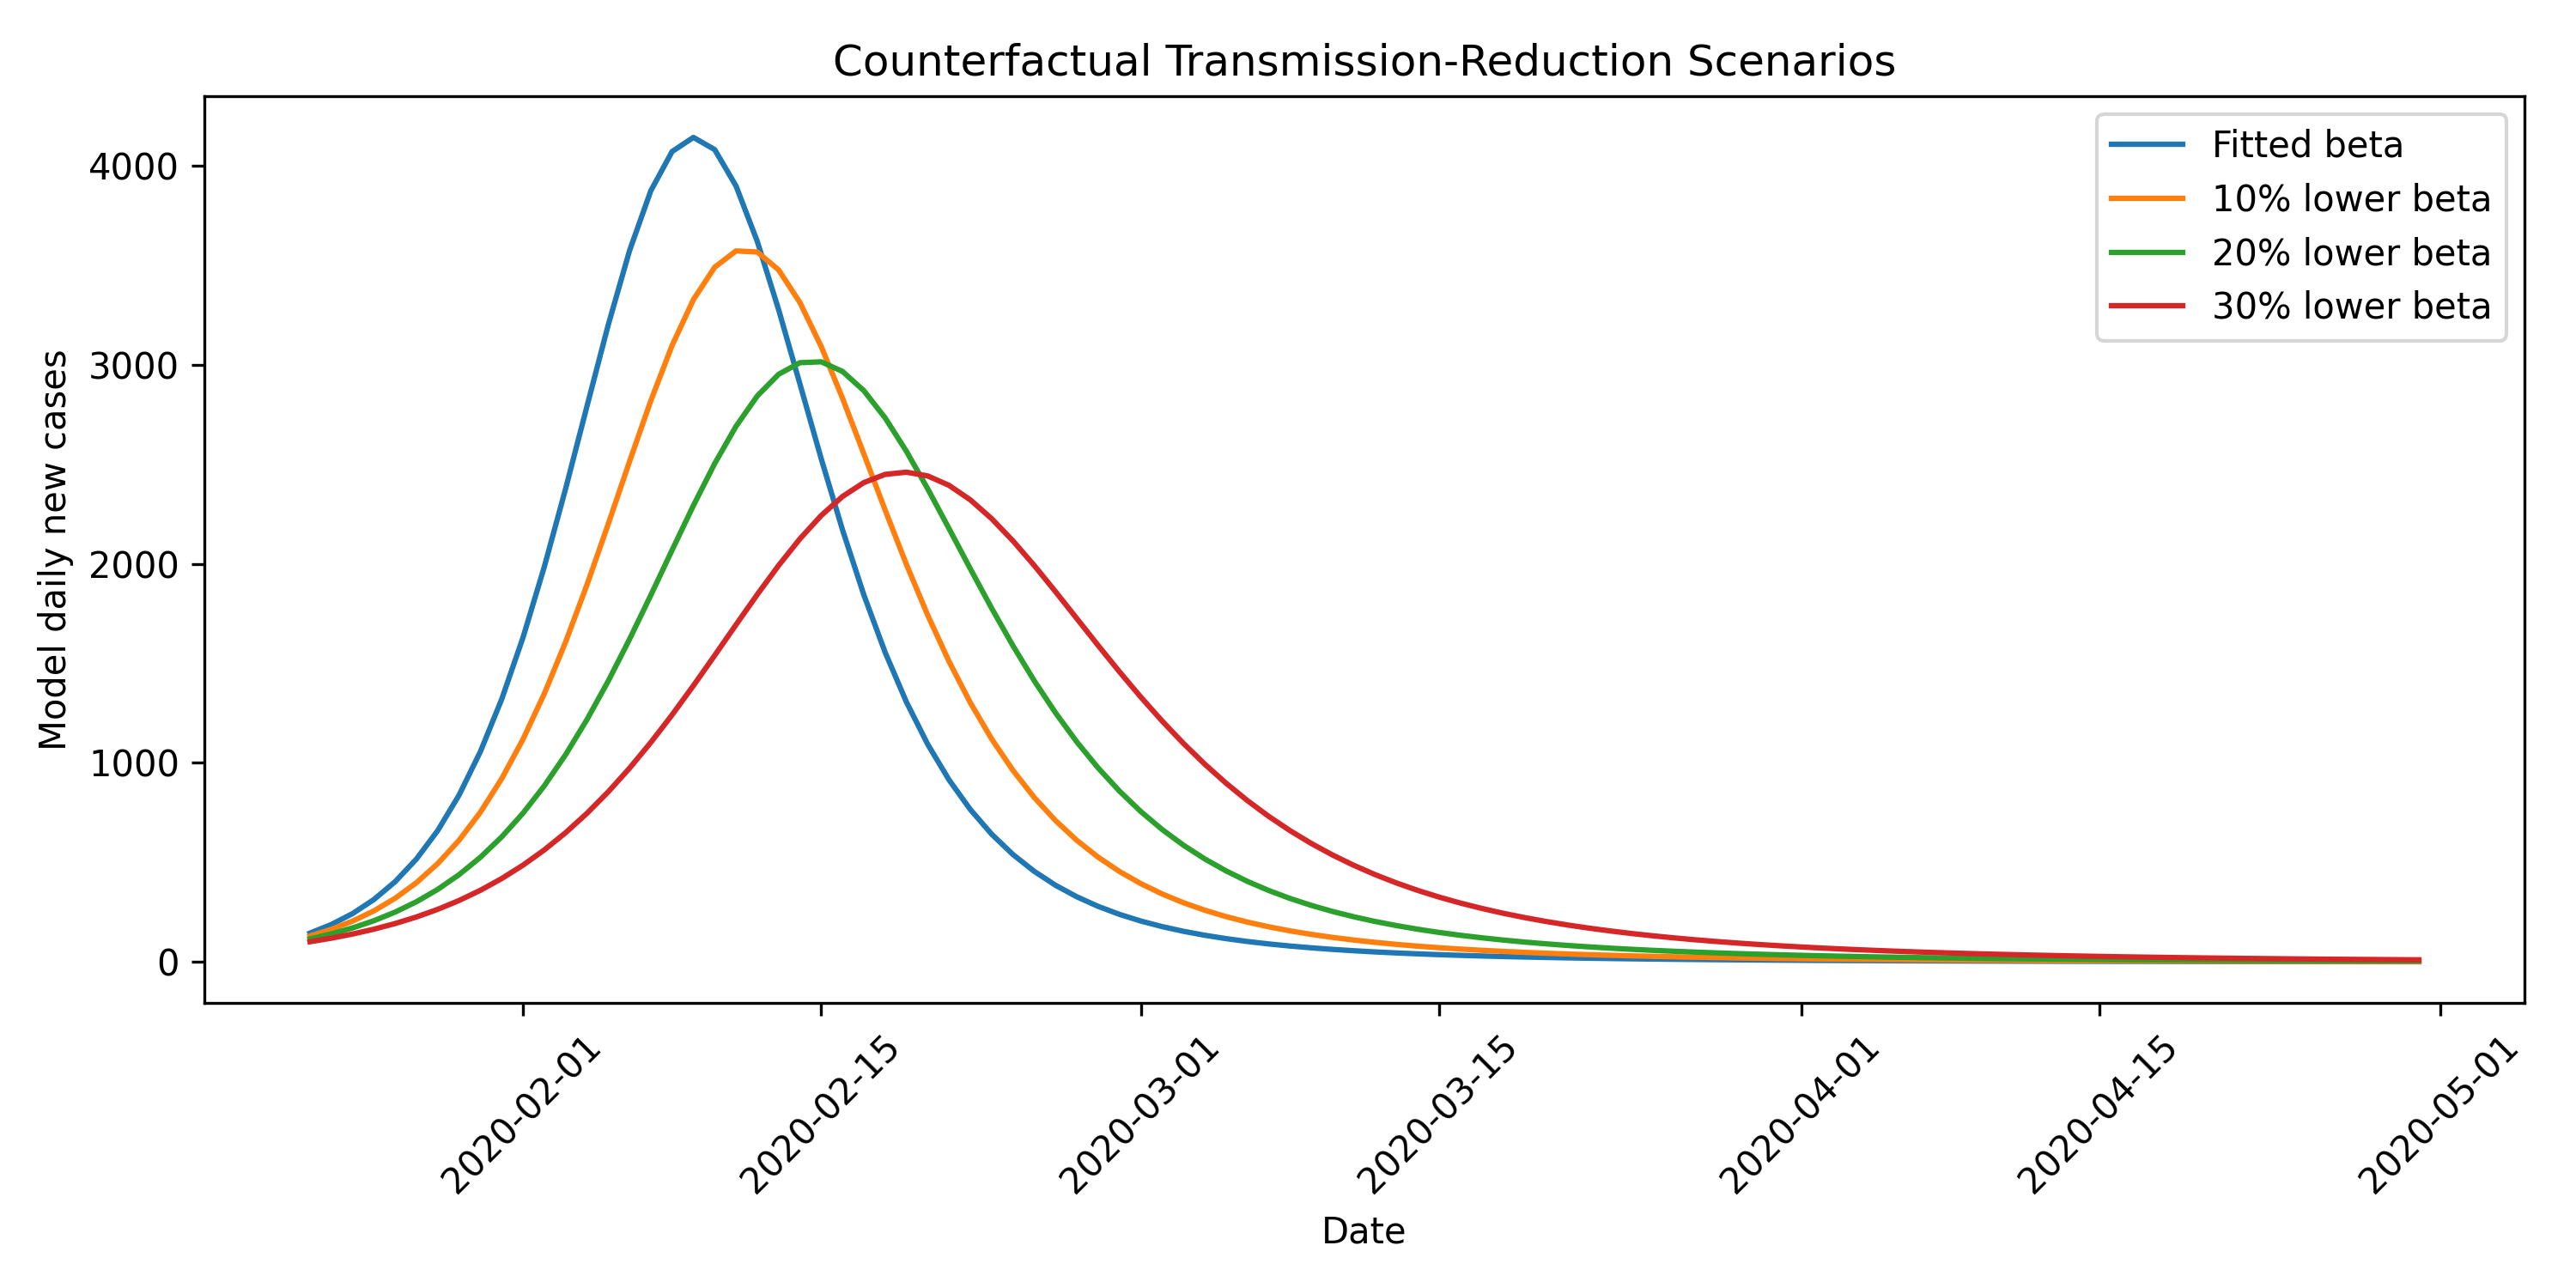
\includegraphics[width=0.9\textwidth]{figures/hubei_counterfactual_scenarios.png}
    \caption{Counterfactual SIR simulations with the fitted transmission rate and 10\%, 20\%, and 30\% lower transmission rates.}
    \label{fig:counterfactual}
\end{figure}

\begin{table}[H]
    \centering
    \begin{tabular}{lrrr}
        \toprule
        Scenario & Peak daily cases & Peak date & Final cumulative cases \\
        \midrule
        Fitted $\beta$ & 4,141 & 2020-02-09 & 68,332 \\
        10\% lower $\beta$ & 3,571 & 2020-02-11 & 68,001 \\
        20\% lower $\beta$ & 3,014 & 2020-02-15 & 67,421 \\
        30\% lower $\beta$ & 2,460 & 2020-02-19 & 66,369 \\
        \bottomrule
    \end{tabular}
    \caption{Summary of transmission-reduction scenarios.}
    \label{tab:scenarios}
\end{table}

The most visible effect is on the peak. A 30\% reduction in $\beta$ lowers the peak from about 4,141 model daily cases to about 2,460 model daily cases, a decrease of about 41\%. The peak also shifts from February 9 to February 19. In this fixed study window, the final cumulative case count also decreases, although less dramatically than the peak.

\section{Discussion and Limitations}

The model supports the idea that reducing transmission can flatten an epidemic curve. In the counterfactual simulations, lower values of $\beta$ produce lower and later peaks. The time-varying model adds another interpretation: the reported first wave is better described when effective transmission is allowed to decrease during the outbreak. This is more realistic than assuming a constant contact or transmission rate for the whole period.

However, this model has several limitations. First, the SIR model assumes homogeneous mixing, so every susceptible individual is treated as equally likely to contact every infected individual. Real COVID-19 spread depends on household structure, age, occupation, travel, and local policy. Second, reported confirmed cases are not the same as true infections. They depend on testing availability, reporting rules, and case definitions. Third, the time-varying $\beta(t)$ curve should not be interpreted as a direct measurement of one specific policy. It is an effective transmission rate inferred from reported case data, so it also reflects reporting changes and model assumptions. Finally, the model does not include exposed but not yet infectious individuals, asymptomatic infection, hospitalization, deaths as a separate compartment, or outside infections. AlQadi and Bani-Yaghoub discuss how adding global dynamics and external infection effects can improve COVID-19 SIR-type models \cite{alqadi2022global}, which highlights why the standard SIR model should be interpreted cautiously.

Overall, the simple SIR model is useful for approximating the broad shape of the first Hubei wave and for testing basic transmission-reduction scenarios. The time-varying version is a better descriptive model, but it is still not detailed enough for real policy forecasting.

\section{Conclusion}

A simple SIR model can approximate the broad cumulative case pattern of the first reported COVID-19 wave in Hubei. Allowing $\beta(t)$ to decline over time improves the fit and gives a more realistic interpretation of changing transmission during the outbreak. In addition, reducing the transmission rate in counterfactual simulations lowers the daily case peak and delays its timing. The project shows how a basic mathematical model can connect real data to a scientific question, while also making clear that reported COVID-19 dynamics are more complicated than the assumptions of a standard SIR system.

\section*{Code Availability}

The code and project files are available in the \href{https://github.com/Hans-Yin/Intro-to-Math-Modeling-Final-Project/}{GitHub repository}.

\bibliographystyle{plainnat}
\bibliography{references}

\end{document}
